\section{Методы, применяемые в работе}
\begin{frame}
    \frametitle{Уравнения состояния}

    \begin{block}[Уравнеие Тейта для жидкости]
         \begin{equation}
             \frac{\hat{\rho} - \rho_0}{\hat{\rho}} = C \log_{10}
             \frac{B + P}{B + P_0}
         \end{equation}
    \end{block}
    \begin{block}[Уравнение идеального газа]
\begin{equation}
    P = \frac{RT}{M} \hat{\rho}
\end{equation}
    \end{block}

\end{frame}

\begin{frame}
    \frametitle{Методы, применяемые в работе}
        \begin{enumerate}
            \begin{columns}
            \begin{column}{0.6\textwidth}
                \item Метод конечных разностей второго порядка для
                    дискретизации по пространству с использованием
                    шахматной сеткой.
                \item Явный метод предиктор-корректор по схеме Хойна
                    для интегрирования по времени.
            \end{column}
            \begin{column}{0.4\textwidth}
                \begin{figure}[H]
                    \centering
                    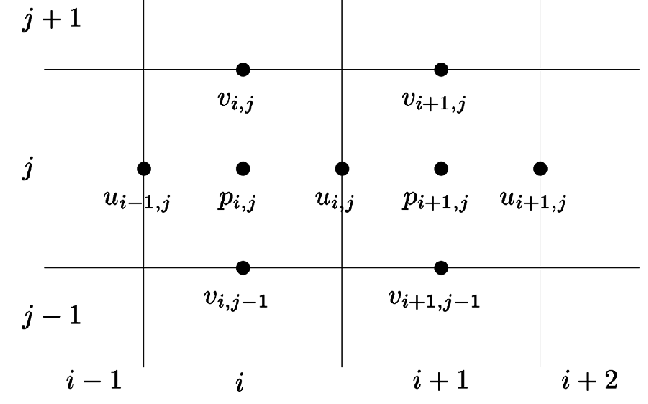
\includegraphics[width=\textwidth]
                    {img/staggered-grid.png}
                \end{figure}
            \end{column}
            \end{columns}
            \item Метод Ньютона-Рафсона для нахождения
                давления и газонасыщенности.
        \end{enumerate}
\end{frame}
